




%\raggedleft
%\textit{
%Cet hiver a des airs de printemps\\
%Des peuples ou de l'esprit, au diable l'âme.\\
%Le vent se lève, ça faisait longtemps\\
%Triste de s'enfermer pour quelques grammes.\\
%}

%\medskip

%\raggedright

%Cet avenir des airs de passé\\
%S'il fallait juste trouver le régime,\\
%Assassinée la complexité\\
%Maintes perspectives se cachent en les crimes.\\

%\medskip
%\raggedleft

%Pour une morphogenèse politique\\
%Adieu le coron, ses tristes briques\\
%Murs qui s'érigent tuent votre espérance.\\

%\medskip
%\raggedright

%Perle de la mer, sirène hante la crique\\
%Du haut des tours s'amuser du cirque\\
%L'hiver d'idées qui peuple la France.\\




%------------------------------------


\newpage






%\chapter*{Conclusion}{Conclusion}
\chapter*{Conclusion}


% to have header for non-numbered introduction
\markboth{Conclusion}{Conclusion}


\headercit{Explorer sans relâche les systèmes géographiques\ldots}{Arnaud Banos}{}



Le lecteur qui aura tenu jusqu'ici et qui a la mémoire solide ou bien sélective, ou encore qui aura adopté un style de lecture roman policier, se plaindra du manque d'originalité dans l'origine des citations introductives. Ce n'est pas anodin si les positions de \noun{Banos}, simples mais efficaces et profondes, ouvrent et ferment ce travail : les ``9 principes de Banos'' sont implicitement présents dans la majorité des travaux menés et perspectives ouvertes. 


\comment[JR]{Le démon de Banos : est capable de faire de l'interdisciplinaire et du disciplinaire sans se perdre, et respecte les 9 points.}



















%%%%%%%%%%%%%%%%%%%%
%% Add epilogue -> may be separated




%\chapter{When Science meets Art}{Quand la science se mêle à l'art} % Chapter title

%\label{app:art} % For referencing the chapter elsewhere, use \autoref{ch:name} 

%----------------------------------------------------------------------------------------


%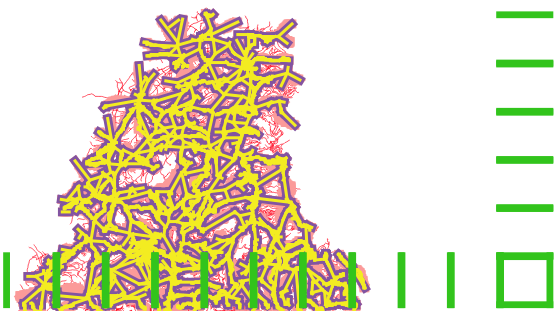
\includegraphics[angle=90]{Figures/Art/Capture d’écran 2016-08-08 à 11.46.55}











